% Phase 2 paper, IEEE two-column conference format, 8 to 10 pages including references.
% Build from docs/paper:  pdflatex main && bibtex main && pdflatex main && pdflatex main
%
% Every number in the paper comes from a generated file in tables/ or figures/ (written by the scripts in
% scripts/ from saved runs in results/), never typed by hand. Until a file exists, \generated{} prints a note.
% \plan{} notes say what each section must contain (Phase 2 brief, Section 5.2); delete each one as the text
% is written. The draft must have no \plan{} left before submission.

\documentclass[conference]{IEEEtran}
\IEEEoverridecommandlockouts

\usepackage[T1]{fontenc}
\usepackage{amsmath,amssymb}
\usepackage{booktabs}
\usepackage{array}
\usepackage{graphicx}
\usepackage{xcolor}
\usepackage{cite}
\usepackage{url}
\usepackage{tikz}
\usetikzlibrary{arrows.meta,positioning}
\usepackage[hidelinks]{hyperref}

\newcommand{\plan}[1]{\textcolor{gray}{\textit{[Plan: #1]}}}
% \generated{file}{what writes it}: input a generated table, or print a note while it does not exist yet.
\newcommand{\generated}[2]{\IfFileExists{#1}{\input{#1}}{\plan{\texttt{\detokenize{#1}}, written by #2}}}
% \generatedfigure{file}{caption}{label}{what writes it}: a one-column figure from a generated PDF, or a note.
\newcommand{\generatedfigure}[4]{\IfFileExists{#1}{\begin{figure}[t]\centering
  \includegraphics[width=\columnwidth]{#1}\caption{#2}\label{#3}\end{figure}}{\plan{\texttt{\detokenize{#1}}, written by #4}}}
\newcommand{\cthree}{C\textsuperscript{3}-Bench}

\begin{document}

\title{Verified Optimization Agents: Requirement-Level Verification and Calibrated Abstention for LLM-Based
Optimization Modeling\\[2pt]
\large Project G1-01, AI4015 Agentic Artificial Intelligence, Fall 2026}

\author{
\IEEEauthorblockN{Mushahid Hussain}
\IEEEauthorblockA{23I-0541 (group head)\\
FAST NUCES, Islamabad\\
i230541@isb.nu.edu.pk}
\and
\IEEEauthorblockN{Muhammad Waqas}
\IEEEauthorblockA{23I-0569\\
FAST NUCES, Islamabad\\
i230569@isb.nu.edu.pk}
\and
\IEEEauthorblockN{Abdul Rauf}
\IEEEauthorblockA{23I-0591\\
FAST NUCES, Islamabad\\
i230591@isb.nu.edu.pk}
}

\maketitle

% ---------------------------------------------------------------------------------------------------------------
\begin{abstract}
Large language models (LLMs) can turn a word problem into solver code, but the code can run, report an optimal
value and still be wrong, and current systems answer every question anyway. We built a multi-agent pipeline that
answers only when its checks pass and otherwise escalates with reasons or abstains. Besides solver feasibility, its
verifier uses three signals that need no reference answer: the share of the question's numbers found in the code,
the share of parsed requirements tied to a named constraint, and whether reworded questions reach the same optimum.
The answer threshold can be calibrated to a target wrong-accept rate with an exact binomial bound. We tested three
pre-registered hypotheses on OPT-Engine problems with gpt-oss-120b and six other models. The signals do tell correct
and wrong models apart: the AUROC goes from 0.54 for feasibility alone to 0.87 (H1 partly supported, in 6 of 7
pre-registered runs). Error control breaks when the problem class changes. At $\alpha = 10\%$ no calibrated
threshold kept the held-out wrong-accept rate on target while answering half the problems (H2 not supported).
Under the same token budget, plain majority voting over resampled answers was at least as accurate for every model.
On 1,457 held-out problems it wrongly accepted 3.6\% of its answers, against 6.4\% for the pipeline at 50\% coverage
(H3 not supported), and combining the two did not beat voting. All code, runs and analysis scripts are released.
\end{abstract}

\begin{IEEEkeywords}
optimization modeling, large language models, multi-agent systems, verification, selective prediction
\end{IEEEkeywords}

% ---------------------------------------------------------------------------------------------------------------
\section{Introduction}
\label{sec:intro}

Operations teams usually describe planning problems in plain language, but solving them needs a formal optimization
model. LLMs can now write these models as solver code, and fine-tuned systems get roughly 60\% to 70\% macro accuracy
on the standard benchmarks~\cite{chen2025sirl,lu2025optmath,huang2025orlm}. Accuracy drops a lot once problems get
larger and more realistic. On the industrial MIPLIB-NL benchmark the best model solves just 39\% of the instances,
and SIRL-32B goes from 87.40\% on MAMO-Complex down to 1.43\%~\cite{li2026miplibnl,shen2024mamo}.

A bigger issue is that these systems always give an answer. Generated code can run, return an ``optimal'' value and
still leave out a requirement that the question states. In the error analyses of OptiTree~\cite{liu2025optitree} and
ORLM~\cite{huang2025orlm}, missing constraints are the most frequent error, and they are also a common modelling error
on MIPLIB-NL~\cite{li2026miplibnl}. Existing checks are weak here: they rely on the same model reviewing
itself~\cite{jiang2025llmopt}, on LLM verdicts that are not calibrated~\cite{liu2026optverifier,zheng2023judging}, or
on solver queries that cannot notice a requirement that was never written~\cite{abdulrahman2026verisimpl}. Verifier
models do help with math reasoning~\cite{cobbe2021gsm8k}, but an uncalibrated verdict gives no guarantee once the data
shifts. In operations, a confident wrong plan is worse than no plan at all: if a crew limit or a capacity is quietly
dropped, the schedule may be impossible to carry out. An operations user needs a system that answers only when its
checks back the answer up, and otherwise abstains or passes the case to an analyst along with the reasons.

Our base paper, OPT-Engine~\cite{chen2026optengine}, studies where LLM-written models break down as problems grow. It
shows that solver-integrated reasoning (SIR) is needed and that extra constraints still pull accuracy down, but it
does not catch failures at run time. After reviewing ten recent papers we found three gaps, and each one gives a
research question:
\begin{itemize}
\item \textbf{Gap~1, label-free verification.} None of the reviewed systems checks at inference time, without
reference answers, whether a model uses every number in the question or reaches the same optimum when the question
is reworded. Self-consistency improves accuracy on general tasks~\cite{wang2023selfconsistency}, but we found no
work that uses it to check paraphrased optimization questions. Checks on the stated requirements exist only partly, as verdicts
on model structure~\cite{liu2026optverifier} and solver queries per constraint~\cite{abdulrahman2026verisimpl}.
\textbf{RQ1:} can these requirement-level signals spot wrong models better than solver feasibility on its own?
\item \textbf{Gap~2, error control under shift.} No reviewed system can decline to answer while keeping its error
rate under control, and in the closest recent attempt the error bound did not hold on new
problems~\cite{lian2026admitor}. Using ideas from selective
classification~\cite{geifman2017selective,geifman2019selectivenet,kamath2020selective}, risk-controlling prediction
sets~\cite{bates2021risk,angelopoulos2021gentle} and conformal prediction~\cite{vovk2005algorithmic,angelopoulos2024conformal},
we ask \textbf{RQ2:} does a threshold calibrated on nine problem classes keep the wrong-accept rate at or under its
target on the unseen tenth class?
\item \textbf{Gap~3, cost.} Frameworks like CAMEL~\cite{li2023camel}, AutoGen~\cite{wu2023autogen} and
MetaGPT~\cite{hong2024metagpt} can do a lot with several agents, but their token use is seldom compared with a single
agent that samples more under the same budget, even though the cost of LLM calls is a known
concern~\cite{chen2024frugalgpt}. \textbf{RQ3:} given the same token budget, does the multi-agent pipeline trade off
accuracy and wrongly accepted answers better than one agent that resamples?
\end{itemize}

\noindent Our contributions are:
\begin{enumerate}
\item a verifier with three label-free signals: number coverage, requirement coverage (each parsed requirement is
linked to a named constraint of the generated model) and paraphrase-optimum agreement, combined with solver
feasibility into one score;
\item a decision layer that answers, abstains or escalates, with a threshold calibrated to a target wrong-accept rate
by an exact binomial bound, tested on held-out problem classes and on OpsOR-Bench, a small set of operations problems
we built as a shift test;
\item a single-agent baseline matched to the pipeline's token use within 10\%, and per-step token accounting
that shows where each system spends its tokens;
\item an open implementation in which every ablation and every number in this paper is computed from saved run
records by a script.
\end{enumerate}

\section{Related Work}
\label{sec:related}

\textbf{Benchmarks.} OPT-Engine~\cite{chen2026optengine} generates problems from parametric generators in ten classes
of linear and mixed-integer programs, so that difficulty can be raised in a controlled way, and computes each optimum
with a solver. It compares pure-text reasoning, text reasoning with computational tools, and SIR, and finds that only
SIR stays reliable as problems grow, while constraint augmentation lowers the accuracy of both pure-text
reasoning and SIR. Writing constraint models from natural language is a long-standing goal~\cite{tsouros2023holy}, and agentic
frameworks apply LLMs to what-if analysis in supply chains~\cite{li2023optiguide}. OptiBench and
ReSocratic~\cite{yang2025optibench} and OptMATH~\cite{lu2025optmath} provide fixed collections and synthesized
training data, NL4Opt~\cite{ramamonjison2022nl4opt} and MAMO~\cite{shen2024mamo} explore natural language formulations,
and MIPLIB-NL~\cite{li2026miplibnl} reverse-builds industrial instances from MIPLIB 2017. Reference
answers are not always reliable: one audit found 50\% of IndustryOR and 41\% of OptMATH-Bench instances
incorrect~\cite{zhang2025optimind}. We therefore use generated problems with computed optima, and check doubtful
references by hand.

\textbf{Training and search.} ORLM~\cite{huang2025orlm} and OptMATH~\cite{lu2025optmath} fine-tune models on
synthesized problems, SIRL~\cite{chen2025sirl} uses the solver as a reward in reinforcement learning,
LLMOPT~\cite{jiang2025llmopt} adds a self-correction loop, and OptiTree~\cite{liu2025optitree} searches over
hierarchical decompositions. All of them raise accuracy, but
all answer every question, and none reports the token cost of its extra calls. The error analyses of these papers
motivate our verifier: missing constraints account for 61.9\% to 82.6\% of the remaining errors of
OptiTree~\cite{liu2025optitree}, and ignored constraints or implicit conditions for 56.3\% of the modelling errors of
ORLM~\cite{huang2025orlm}.

\textbf{Verifying generated models.} Opt-Verifier~\cite{liu2026optverifier} asks LLMs for binary verdicts on a
model's structure. It reaches 68\% recall on hard structure errors, ignores numerical values, and uses about nine
calls and 5,300 to 8,500 tokens per problem. VeriSimpl~\cite{abdulrahman2026verisimpl} queries the solver on
simplified versions of the problem; its precision of 78.5\% to 91.5\% comes with a recall of only 23.0\% to 34.2\%, and
its queries cannot detect a requirement that the program omits entirely. ReLoop~\cite{lian2026reloop} and a
falsification-based test battery~\cite{li2026falsification} change the input data of a generated model and test
whether the solver's answer responds as the text implies. These checks find real errors, but none of them is turned
into a rule for refusing to answer at a known error rate.

\textbf{Answering with an error guarantee.} AdmitOR~\cite{lian2026admitor} is the closest work. It answers,
abstains or escalates using the agreement of three model families, with a finite-sample bound on wrong acceptances.
The bound held on its calibration problems but failed on a benchmark stream, where 22 of 138 accepted answers
(15.9\%) were wrong, against a 5\% target. The authors trace 20 of the 22 cases to questions that omit needed numbers
or print them with too little precision; their check for values missing from the text flags 9 of the 15
omitted-number cases. This result motivates two choices in our design: a data-level signal (number coverage) and an
error bound that is always tested on problem types the calibration has not seen. Table~\ref{tab:related} compares
the closest systems with ours.

\begin{table}[t]
\centering
\caption{Closest work compared with ours. ``Refuses'': the system can decline to answer with a target error rate.
``Shift'': that error control is tested on problems unlike the calibration set. ``Tokens'': the paper reports the LLM tokens its check costs (ReLoop only as about three times the base cost; the test battery only its solver time).}
\label{tab:related}
\footnotesize
\setlength{\tabcolsep}{3pt}
\begin{tabular}{@{}>{\raggedright\arraybackslash}p{2.05cm}>{\raggedright\arraybackslash}p{2.55cm}ccc@{}}
\toprule
\textbf{System} & \textbf{Check at inference} & \textbf{Refuses} & \textbf{Shift} & \textbf{Tokens} \\
\midrule
Opt-Verifier~\cite{liu2026optverifier} & LLM verdicts on structure & no & -- & yes \\
VeriSimpl~\cite{abdulrahman2026verisimpl} & solver queries on simplified problems & no & -- & no \\
ReLoop~\cite{lian2026reloop} & responses to changed data & no & -- & partly \\
Test battery~\cite{li2026falsification} & sound test batteries & no & -- & no \\
AdmitOR~\cite{lian2026admitor} & agreement of three model families & yes & yes & no \\
\textbf{Ours} & number and requirement coverage, agreement of rewordings & yes & yes & yes \\
\bottomrule
\end{tabular}
\end{table}

\section{Problem Formulation}
\label{sec:problem}

\textbf{Task.} The input is a question $q$ in natural language that states an optimization problem together with all
its data. The system returns a tuple $(\hat{a}, d, e)$: a predicted optimal value $\hat{a} \in \mathbb{R} \cup
\{\varnothing\}$, a decision $d \in \{\textit{answer}, \textit{abstain}, \textit{escalate}\}$ and a short explanation
$e$ for the user. It abstains when it cannot build a model that the solver finds feasible and optimal, and escalates
when it has such a model but its checks do not support it, giving the failed checks as reasons. Only an answered value
is shown as a result.

\textbf{Correctness.} With the reference optimum $y$, a value is correct when $|\hat{a} - y| \le 0.002\,|y|$, the rule
of the base paper's evaluation code~\cite{chen2026optengine}. Correctness is used only for evaluation; the system never
sees $y$.

\textbf{Score and decision.} The verifier gives each problem a score $S(q) \in [0, 1]$ from label-free signals, and
$S(q) = 0$ when no feasible model exists. For a threshold $\tau$ the system answers when the model is feasible and
$S(q) \ge \tau$. Over a set of $N$ problems with answered set $A_\tau$,
\begin{equation}
\mathrm{coverage}(\tau) = \frac{|A_\tau|}{N}, \qquad
\mathrm{WAR}(\tau) = \frac{|W_\tau|}{|A_\tau|},
\end{equation}
where $W_\tau \subseteq A_\tau$ holds the answered problems whose value is wrong. WAR is the wrong-accept rate and
$1 - \mathrm{WAR}$ the selective accuracy. A system that never abstains, such
as the SIR baseline, answers whenever the solver returns an optimal status, so its coverage is its share of models
solved to optimality.

\textbf{Calibration.} Given a target $\alpha$, the threshold is chosen on calibration problems only. Candidate
thresholds are scanned in a fixed order from strict to lenient, and the scan stops before the first one whose one-sided
exact 95\% upper bound on the calibration wrong-accept rate exceeds $\alpha$; the fixed order keeps the bound valid
across thresholds. A threshold needs at least 29 accepted problems, since with fewer even zero wrong answers cannot
give a bound below 10\%. When no threshold passes, the system answers nothing. It is tested
leave-one-class-out: calibrated on nine of the ten problem classes and applied to the tenth, so that each problem is
scored once, in the fold that holds out its class.

\textbf{Cost.} Every LLM call is metered in input and output tokens. Two systems are compared at an equal budget when
their mean tokens per problem differ by at most 10\%.

\textbf{Hypotheses.} Each research question has one testable prediction.
\begin{itemize}
\item \textbf{H1.} Adding the signals to feasibility raises the area under the ROC curve (AUROC) for separating correct
from wrong answers by at least 0.10, and removing any one signal lowers it.
\item \textbf{H2.} With $\alpha = 10\%$, the pooled held-out wrong-accept rate is at most $\alpha$, reported with its
exact 95\% interval, while at least 50\% of all problems are answered.
\item \textbf{H3.} With $k = 3$ reworded runs, the pipeline's wrong-accept rate at 50\% coverage is lower than that of
the single-agent baseline B2, which keeps sampling answers until it reaches the pipeline's mean token budget. It counts
as met only if the 95\% bootstrap interval of the paired difference at $k = 3$ is entirely below zero.
\item \textbf{H3c} (pre-registered after H3 failed; repository issue \#103). The pipeline runs at $k = 1$, B2 samples use
the rest of the budget, and the score is the mean of the pipeline's score and the share of B2 samples that agree with
its answer. Its WAR at 50\% coverage is lower than B2's, again with the whole paired interval below zero.
\end{itemize}

\section{Proposed System}
\label{sec:system}

\subsection{Agent Roles and Modeling Pipeline}
Five roles exchange structured data (Fig.~\ref{fig:architecture}):

\begin{figure}[t]
\centering
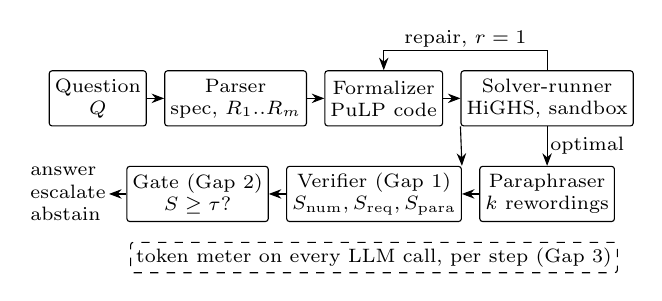
\begin{tikzpicture}[font=\scriptsize, node distance=3mm and 2.2mm,
  box/.style={draw, rounded corners=1pt, align=center, inner sep=2pt, minimum height=7mm},
  result/.style={align=left, inner sep=1pt}, >={Stealth[length=1.6mm]}]
\node[box] (q) {Question\\$Q$};
\node[box, right=of q] (parse) {Parser\\spec, $R_1..R_m$};
\node[box, right=of parse] (form) {Formalizer\\PuLP code};
\node[box, right=of form] (solve) {Solver-runner\\HiGHS, sandbox};
\node[box, below=5mm of solve] (para) {Paraphraser\\$k$ rewordings};
\node[box, left=of para] (ver) {Verifier (Gap 1)\\$S_{\text{num}}, S_{\text{req}}, S_{\text{para}}$};
\node[box, left=of ver] (gate) {Gate (Gap 2)\\$S \ge \tau$?};
\node[result, left=of gate] (dec) {answer\\escalate\\abstain};
\draw[->] (q) -- (parse);
\draw[->] (parse) -- (form);
\draw[->] (form) -- (solve);
\draw[->] (solve.north) -- ++(0,2.5mm) -| node[pos=0.25, above, inner sep=1pt] {repair, $r = 1$} (form.north);
\draw[->] (solve) -- node[right, inner sep=1pt] {optimal} (para);
\draw[->] (solve.south west) -- (ver.north east);
\draw[->] (para) -- (ver);
\draw[->] (ver) -- (gate);
\draw[->] (gate) -- (dec);
\node[draw, dashed, rounded corners=1pt, inner sep=2pt, below=2.5mm of ver] {token meter on every LLM call, per step (Gap 3)};
\end{tikzpicture}
\caption{The pipeline. Each rewording is formalized and solved on its own; B2 instead resamples B1 up to the same
token budget.}
\label{fig:architecture}
\end{figure}

\textbf{1. Structured Parser.} The parser writes a solver-independent specification without solving: the objective
sense and statement, the decision variables with their domains, the parameters with values and units, and a checklist
of requirements $\mathcal{R} = \{R_1, \dots, R_m\}$, each one restriction.

\textbf{2. Formalizer with Targeted Self-Repair.} The formalizer reads $Q$ and the specification and writes PuLP code, naming each constraint after its requirement (e.g., \texttt{R1\_capacity}). If the code fails or the model is not optimal, the code and the error are sent back for up to $r$ repair rounds ($r = 1$ by default).

\textbf{3. Sandboxed Solver-Runner.} The code runs in a separate Python process in isolated mode (\texttt{-I}) with a minimal environment, so no API key is visible to it. HiGHS has a 120-second limit, and the process is stopped after 180 seconds. The runner returns the status $s \in \{\text{optimal}, \text{infeasible}, \text{unbounded}, \text{error}, \text{no\_code}\}$, the objective value $v^*$ and the run time.

\textbf{4. Paraphraser.} When the main model is optimal, the system writes $k$ rewordings of $Q$ (by default $k=3$, at
$T=0.7$); each is formalized and solved on its own, giving optima $v^{(1)}, \dots, v^{(k)}$, and a failed rewording
is retried once.

\textbf{5. Decision Gate and Explainer.} The gate answers, escalates or abstains (Section~\ref{sec:gate}); the
explainer summarizes an accepted model, or lists the failed checks of an escalated one.

\subsection{Label-Free Verification Signals (Gap 1)}
Without reference answers, the verifier computes three signals:

\textbf{Number Coverage ($S_{\text{num}}$).} A number missing from the code often means a missing constraint. Let $\mathcal{N}_Q$ be the numbers in $Q$ (we skip 0, 1 and item labels like ``Package 3'', and treat 24\% and 0.24 as the same) and $\mathcal{N}_C$ the numbers in the code. Then
\begin{equation}
S_{\text{num}} = \frac{|\mathcal{N}_Q \cap \mathcal{N}_C|}{|\mathcal{N}_Q|}.
\end{equation}

\textbf{Requirement Coverage ($S_{\text{req}}$).} Let $\mathcal{R}_{\text{linked}} \subseteq \mathcal{R}$ be the requirements that some constraint of the final model is named after. Then
\begin{equation}
S_{\text{req}} = \frac{|\mathcal{R}_{\text{linked}}|}{|\mathcal{R}|}.
\end{equation}

\textbf{Paraphrase Agreement ($S_{\text{para}}$).} Rewording the question should not change the optimum of a correct model. We compare each rewording that solves to optimality (one that fails twice is dropped and logged) with the main optimum $v^*$, using a relative tolerance of 0.2\%: $|v^{(j)} - v^*| \le 0.002 \cdot \max(|v^*|, |v^{(j)}|)$. $S_{\text{para}}$ is the fraction of solved rewordings that agree. If none solves, or $k = 0$, this signal is not used.

\textbf{Combined Verification Score ($S$).} For an optimal model, $S \in [0, 1]$ is the mean of the available signals, $(S_{\text{num}} + S_{\text{req}} + S_{\text{para}})/3$ in the full pipeline; without the parser or the rewordings that signal is left out. Without an optimal model, $S = 0$.

\subsection{Decision Gating and Error Control (Gap 2)}
\label{sec:gate}
Given the solver status $s$, the score $S$ and a threshold $\tau$, the gate decides
\begin{equation}
d = \begin{cases}
\text{answer}, & \text{if } s = \text{optimal} \text{ and } S \ge \tau, \\
\text{escalate}, & \text{if } s = \text{optimal} \text{ and } S < \tau, \\
\text{abstain}, & \text{if } s \ne \text{optimal}.
\end{cases}
\end{equation}
We either fix the threshold at $\tau = 0.8$ or calibrate it to a target $\alpha$ as in Section~\ref{sec:problem}.

\subsection{Token Accounting and Efficiency Metering (Gap 3)}
For every LLM call, a token meter logs the input and output tokens, the latency and the calling role. Run records store these per step (\texttt{RunRecord.usage\_by\_step}), which lets us compare the pipeline and a single agent at the same budget.

\section{Experimental Setup}
\label{sec:setup}

\subsection{Benchmarks and Problem Splits}
\textbf{1. OPT-Engine (\cthree{}).} OPT-Engine~\cite{chen2026optengine} has ten problem classes: BinPacking, Inventory, JobShop, Knapsack, NetworkFlow, Pollution, Portfolio, Production, TSP and Transportation. We use fixed samples:
\begin{itemize}
\item \texttt{canonical\_200}: 20 problems per class, for the main repeats and the baselines.
\item \texttt{canonical\_587}: \texttt{canonical\_200} plus up to 40 more problems per class, a larger calibration
sample.
\item \texttt{constraint\_pairs\_60} (60 pairs, 120 problems) and \texttt{linguistic\_60}: added constraints and
varied wording.
\item \texttt{canonical\_587\_rest\_387} and \texttt{canonical\_unused}: the 387 problems of \texttt{canonical\_587}
outside \texttt{canonical\_200}, and the 1,070 canonical problems in no other sample (half of them BinPacking), used
only for the pre-registered tests (1,457 held-out problems together).
\item \texttt{ablation\_50}: for the ablations, 5 of the 20 problems per class of \texttt{canonical\_200}.
\item \texttt{dev\_30} and \texttt{dev\_93}: development splits (3 and about 10 problems per class), used only to design prompts and study errors, never for reported results.
\end{itemize}

\textbf{2. OpsOR-Bench.} To test shift (H2) we wrote OpsOR-Bench, 36 problems from three operations families: gate assignment, ground-crew rostering and equipment dispatch (\texttt{scripts/make\_opsor.py}). Their structure and wording differ from anything the OPT-Engine generators produce.

\subsection{Evaluated Models and Baselines}
All models run on open-weight endpoints in Amazon Bedrock:
\begin{itemize}
\item \textbf{Primary Model:} \texttt{openai.gpt-oss-120b-1:0}, an open-weights mixture-of-experts model used for all pipeline roles and baselines.
\item \textbf{Second Paraphrase Model:} \texttt{deepseek.v3.2}, used for the B0 baseline comparison and to test whether an independent model family improves paraphrase agreement.
\item \textbf{Six more models} for the pre-registered tests: DeepSeek V3.2, Qwen3 Next 80B, Mistral Large 3, Kimi
K2.5, GLM 4.7 and gpt-oss-20b. Each one plays every pipeline role and also runs B1 and B2 on \texttt{canonical\_200}.
We fixed this list after a smoke test on two problems, before any full run.
\item \textbf{Solver:} HiGHS through PuLP 3.3.2 on Python 3.12 (\texttt{pulp.HiGHS(msg=False, timeLimit=120)}).
\end{itemize}

We compare the pipeline with three reference systems:
\begin{itemize}
\item \textbf{Baseline B0 (Direct SIR):} single-turn SIR as in the base paper. The model writes PuLP code for $Q$; an optimal result gives the answer, and anything else is a failure.
\item \textbf{Baseline B1 (SIR with Self-Repair):} B0 plus up to $r = 1$ repair round, triggered by a solver error traceback or a non-optimal status.
\item \textbf{Baseline B2 (Budget-Matched Single Agent):} it starts as B1 and keeps drawing new samples at $T = 0.7$ until it has spent the pipeline's mean tokens at $k = 3$ (about 20,800 per problem; for the six other models 1.25 times their pipeline's mean, trimmed back to the pipeline's tokens in the analysis). Its answer is the most common optimum, and its score is the share of samples that agree with it.
\end{itemize}

Formalizer calls use $T = 0$ and the paraphraser $T = 0.7$. Where there are several repeats we report their mean and
sample standard deviation. No model, prompt or repair round ever sees a reference answer.

\section{Evaluation Methodology}
\label{sec:methodology}

Accuracy is the share of all problems answered correctly under the 0.2\% rule of Section~\ref{sec:problem}, and
coverage and the wrong-accept rate (WAR) are as defined there. Every WAR at a calibrated threshold is reported with
its exact two-sided 95\% Clopper-Pearson interval, and every AUROC of the score $S$ with 1,000 bootstrap resamples.
H2 uses the leave-one-class-out calibration of Section~\ref{sec:problem} (\texttt{scripts/analyze\_gap2.py}). H3 and
H3c compare the systems when each answers its top 50\% of problems by score (for H3, ties broken at random over
1,000 draws), and report the paired bootstrap interval of the WAR difference and McNemar's test on accuracy
(\texttt{scripts/analyze\_e3.py}, \texttt{scripts/explore\_combination.py}). The analysis scripts read only saved
run records, so every number can be recomputed without API calls.


\section{Results}
\label{sec:results}
Each subsection reports one experiment, and Table~\ref{tab:gap_resolution} gives every verdict. Unless stated, the
model is gpt-oss-120b and the threshold is 0.8.
\generated{tables/gap_resolution.tex}{scripts/make\_paper\_tables.py}

\subsection{Baselines and the base paper (E1, E2)}
\generated{tables/baselines.tex}{scripts/compare\_baselines.py}
Over three repeats, B0 and B1 reach 78.5\% and 79.5\% on \texttt{canonical\_200} (Table~\ref{tab:baselines}). Where
the base paper reports SIR accuracy, our B0 is close to it or above it (Knapsack 98.3\% against 93.2\%, NetworkFlow
96.7\% against 100\%, TSP 95.0\% against 85.9\%), and DeepSeek V3.2, the
base paper's model, reaches 77.0\% as B0. Every system scores 0\% on Pollution, whose references the stated model
cannot reproduce (Section~\ref{sec:references}).

\subsection{Gap 1: do the signals detect wrong models? (H1)}
\generated{tables/gap1.tex}{scripts/analyze\_gap1.py}
The combined score separates correct from wrong answers with an AUROC of 0.87 over three repeats, against 0.54 for
feasibility alone (Table~\ref{tab:gap1}), and the mean gain is at least 0.28 on every sample of that table. Paraphrase agreement
carries most of it (0.85 alone); number coverage barely separates (0.55) and requirement coverage adds little (0.64). H1
is therefore partly supported: the gain holds, but removing a signal does not always lower the AUROC
(Section~\ref{sec:ablations}). In the pre-registered runs the gain is 0.187 to 0.305 for six of seven, and 0.075 for
gpt-oss-20b, whose feasibility alone already gives 0.86 (Table~\ref{tab:preregistered}).

\subsection{Gap 2: calibrated abstention and the shift test (H2)}
\generated{tables/gap2.tex}{scripts/analyze\_gap2.py}
No calibration meets H2 (Table~\ref{tab:gap2}). At $\alpha = 10\%$ the leave-one-class-out thresholds answer 10.3\% of
\texttt{canonical\_200} and 15.7\% of \texttt{canonical\_587}, and on the 1,070 unused problems 47.5\% with 15.9\%
wrong; the smallest $\alpha$ the data can meet is 12\% to 21\%. The cause is a floor in the score: on
\texttt{canonical\_587}, 21 of the 280 answers with the top score 1.0 are wrong, among them all 10 Pollution answers
and 8 of 54 Production answers, misreadings that every rewording repeats. A threshold calibrated on the other classes
cannot exclude them. Without Pollution (the sensitivity analysis), the fixed threshold 0.8 answers 86\% to 89\% of the
problems at a WAR of 5.0\% to 5.5\%. On OpsOR-Bench, a threshold calibrated on all classes of \texttt{canonical\_200}
answers nothing at $\alpha = 10\%$ in two of three repeats, while the fixed threshold answers 34 of 36 problems with
no wrong answer; this shift test is weak, because its only two wrong models are infeasible and so never answered.
Figure~\ref{fig:gap2_risk} shows the wrong-accept rate of each repeat at every coverage.
\generatedfigure{../../results/gap2/canonical_200/risk_coverage.pdf}{Wrong-accept rate against coverage of the
pipeline (gpt-oss-120b) on \texttt{canonical\_200}, one curve per repeat, with the fixed threshold 0.8 and the leave-one-class-out
result at $\alpha = 10\%$ (a repeat that answers nothing has no point); the dashed line is $\alpha$}{fig:gap2_risk}{scripts/analyze\_gap2.py}

\subsection{Gap 3: the pipeline against a single agent at an equal token budget (H3)}
\generated{tables/gap3.tex}{scripts/analyze\_e3.py}
On \texttt{canonical\_200} the two systems are close at every $k$ (Table~\ref{tab:gap3}): at $k = 3$, accuracy is
78.0\% against 80.5\% for B2 (McNemar $p = 0.30$), and the WAR at 50\% coverage is 6.0\% against 6.4\%, with an
interval of $[-5.0, +4.3]$ points. Figures~\ref{fig:gap3_cost} and~\ref{fig:gap3_risk} show accuracy against cost and
the wrong-accept rate against coverage for one run of each system. The pre-registered tests on new problems and
models (Table~\ref{tab:preregistered}) give a clearer answer. On all of \texttt{canonical\_587} B2 is 3.1 points more
accurate (McNemar $p = 0.006$), and on the 1,457 held-out problems it wrongly accepts 3.6\% of its answers against
6.4\% for the pipeline, $[+1.6, +4.4]$; its agreement rate is also the better score (AUROC 0.89 against 0.82 on the
387 new problems). B2 is at least as accurate for every model, by 1 to 17 points. For four of the six other models
the pipeline's WAR is the lower one, but no interval excludes zero with 200 problems. H3 is not supported. The
combination of H3c lowers the pipeline's WAR for gpt-oss-120b (significantly only on the 1,070 problems) but raises
it for four of the six other models, and no interval against B2 is below zero: the combination still returns the pipeline's answer and only changes
which answers are accepted. In the
sensitivity analysis only one verdict changes: H3 for GLM 4.7, which we report as a lead, not a finding.
\generatedfigure{../../results/gap3/canonical_200/accuracy_cost.pdf}{Accuracy against mean tokens per problem for
the pipeline and B2 at $k = 1, 2, 3$, with B0 and B1, on \texttt{canonical\_200} with
gpt-oss-120b}{fig:gap3_cost}{scripts/plot\_e3.py}
\generatedfigure{../../results/gap3/canonical_200/risk_coverage_k3.pdf}{Wrong-accept rate against coverage for the
pipeline and B2 (gpt-oss-120b) at $k = 3$ on \texttt{canonical\_200}; the dashed line is the 50\% coverage of H3}{fig:gap3_risk}{scripts/plot\_e3.py}
\generated{tables/preregistered.tex}{scripts/make\_paper\_tables.py from results/preregistered}

\section{Ablation and Comparative Analysis}
\label{sec:ablations}
\generated{tables/ablations.tex}{scripts/ablation\_table.py}
\textbf{Components (E5).} On \texttt{ablation\_50} (Table~\ref{tab:ablations}) the paraphrase check carries the
system: without it the WAR rises from 5.6\% to 14.1\% and the AUROC falls from 0.91 to 0.69, while the tokens fall
from 21,381 to 8,389. Removing number or requirement coverage moves the WAR by at most 1.5 points, and without
requirement coverage the AUROC is even higher (0.93), so not every signal is needed. The parser costs 22\% of the
tokens (16,594 without it) for no gain in accuracy. One repair round raises accuracy from 77.3\% to 82.0\%, and a
second does not help (80.0\%, WAR 9.5\%, one repeat). Two rewordings give the same WAR as three for 80\% of the tokens. The calibrated threshold answers
only 3.3\% of the problems, the H2 result again.

\generated{tables/efficiency.tex}{scripts/efficiency.py}
\textbf{Efficiency and reliability (E6).} The pipeline uses 6 to 8 times the tokens of B1 and about 8 LLM calls per
problem (Table~\ref{tab:efficiency}); for gpt-oss-120b this is US\$8.77 against US\$1.19 per 1,000 problems. No run
failed: the failed-run rate is 0\% for every model and system, below the 5\% target. Solver errors are rare except
for Qwen3 and GLM 4.7 (11\% to 17\% of B1's calls), and repair recovers 24\% to 84\% of the pipeline's problems whose
first model was not optimal. For the six added models, B2 spends more than the pipeline in this
table because it was run to 1.25 times the pipeline's budget; the H3 tests cut it back to the pipeline's tokens.

\section{Failure Analysis}
\label{sec:failures}


Every wrong final answer and every false alarm of the first E3 repeat (\texttt{canonical\_200},
\texttt{constraint\_pairs\_60} and \texttt{linguistic\_60}) was labelled with a failure category, using \texttt{scripts/failure\_analysis.py}, which writes the evidence that needs no judgement (solver status,
the gap to the reference and its direction, the objective sense) next to a hand-assigned label. Of the 380 problems,
102 final answers were wrong. The pipeline refused 78 of them (escalated or abstained) and accepted 24. It also
escalated 20 correct answers (false alarms); 19 of these came from disagreeing rewordings.

\generated{tables/failures.tex}{scripts/make\_paper\_tables.py from results/failures}

\textbf{Wrong constraints, mostly in Inventory and TSP.} Table~\ref{tab:failures} counts 53 wrong constraints:
Inventory 31, TSP 17, Production 3, BinPacking and Knapsack 1 each. Most Inventory models check the storage capacity
only on the closing stock, while the text says it holds at any moment; adding the capacity after each arrival to the
same code gives the reference. The 26 doubtful references are the 20 Pollution answers and 6 Inventory ones
(Section~\ref{sec:references}). All 16 infeasible models are TSP models with a wrongly written
Miller-Tucker-Zemlin subtour constraint. Fourteen apply it to every pair of cities, the start city included, which
rules out every complete tour; two apply it to undirected edges, which forces $u_i < u_j$ and $u_j < u_i$ at once.
For 10 of the 14, leaving the start city out of that one constraint makes the same code return the reference value.
The repair round sees an infeasible status but does not find the cause, so these problems are refused rather than
answered. A repair prompt that names common causes of infeasibility is a direct fix.

\textbf{A misreading that every rewording shares.} Three Production problems were answered with revenues 21 to 31
times the reference. The question gives the handling time of each cargo type on each vehicle; the benchmark means
that every ton uses time on all vehicles, while the model assigns cargo to vehicles. In two of the three cases all
three rewordings repeat the reading, so paraphrase agreement is complete and the score is 1.0. This is the main limit
of the agreement signal: it detects errors that depend on the wording, not errors that every reading of the question
makes. In the third case one rewording found the reference with its sign flipped, but the score of 0.889 still passed
the threshold.

\textbf{Correct refusals.} In constraint-0864 (``if crate 3 is loaded, the capacity drops by 10 kg'') the model
reached 4,181 while all three rewordings reached the reference 4,118, so the answer was escalated with that reason;
the two Knapsack models with continuous items were refused the same way.

\textbf{False alarms.} Of the 20 correct answers that were escalated, 19 failed on paraphrase agreement: a rewording
changed a detail and so reached a different optimum; the other failed on an unused number. This is the cost of the agreement
signal, and it falls on coverage, not on the wrong-accept rate.

\subsection{Case Studies and Trajectories}
\label{sec:case_studies}
Traces of development runs (\texttt{logs/sample/}, \texttt{docs/failures/trajectories.md}) show each path. In a
repair (Portfolio, canonical-1250) the first code raises a \texttt{KeyError}; the repair round fixes it and the
answer is accepted with $S = 0.987$. In a correct refusal (JobShop, canonical-0890) the model reaches 265 while all
three rewordings reach the reference 54, so $S_{\text{para}} = 0$ and the case is escalated. In a wrong accept
(Pollution, canonical-1601) all rewordings agree but two requirements have no named constraint ($S_{\text{req}} =
0.6$), and the mean $S = 0.867$ still passes 0.8; this problem is infeasible as stated, so its reference is doubtful
too.

\subsection{Reference answers}
\label{sec:references}
Pollution and Inventory account for 65 of the 102 wrong answers, and for 18 of the 24 wrong answers that were
accepted, so we checked their references. \texttt{scripts/check\_references.py} reads each question's data from its text,
solves the model the text states with HiGHS, and compares the optimum with the reference (no LLM is used).
\begin{itemize}
\item \textbf{Pollution:} the stated model reproduces none of the 73 references we could read. We also tried four
other readings of the text, and only one of them matched a single reference (canonical-1623), most likely by chance.
Six problems have no feasible solution as written, and 34 references sit below the stated model's optimum, which a
stricter reading could never explain. In 7 of the pipeline's 21 Pollution answers, our answer matches the stated
model's optimum digit for digit. So these references come from a model that the text does not describe.
\item \textbf{Inventory:} 159 of the 160 references are reproduced, and all of them need the capacity to hold right
after a delivery arrives (``at any moment''). A model that checks it only at the end of the day is therefore really
wrong. Two questions say ``at the end of any day'' (canonical-0644 and 0667), and there only the stricter rule gives
the reference. We solved the last one, canonical-0648, by hand (repository issue \#40): the stated model gives 876 or
1,061, but the reference is 1,818, so the reference is wrong.
\end{itemize}
The hand check (\nolinkurl{results/reference_check/hand_labels.csv}) labels 157 Inventory references correct,
canonical-0644 and 0667 ambiguous and canonical-0648 wrong, and confirms by hand that the checked Pollution
references are wrong. Following our protocol, every result is reported with all problems, and the sensitivity
analysis leaves out Pollution and canonical-0648 and keeps the ambiguous problems; no problem is dropped silently.

\section{Limitations and Threats to Validity}
\textbf{Data.} \cthree{} problems are generated from templates, so wording and structure repeat within a class, and
results may not carry over to industrial models such as MIPLIB-NL. The reference check of
Section~\ref{sec:references} shows that the benchmark's own answers are not always reproducible from the question:
every Pollution reference and a few Inventory references follow a model the text does not state. Our tolerance-based
grading therefore counts some correct models as wrong, which lowers the measured accuracy and raises the measured
wrong-accept rate of every system alike.

\textbf{Method.} Number coverage is nearly saturated on this benchmark: in five development runs (four in
\texttt{results/dev\_requirement\_coverage/} and one on \texttt{dev\_30}), 134 of 147 feasible models (91\%) use every
number, and so do all 30 wrong ones, because the generated questions never omit data; on \texttt{canonical\_200} 88\%
of the feasible models do. Paraphrase agreement
cannot detect a misreading that every rewording shares (the Production cases of Section~\ref{sec:failures}).

\textbf{Evaluation.} The exact bound behind the calibrated threshold needs many accepted calibration answers: at a
true wrong-accept rate of 8\%, certifying 10\% needs 593 of them (\texttt{scripts/power\_h2.py}), about four times
what one fold of \texttt{canonical\_200} provides. We therefore added \texttt{canonical\_587}; this is a deviation
from the Phase~1 plan, made after H2 failed on \texttt{canonical\_200}, and both results are reported. The main
configuration uses one model (gpt-oss-120b); the six other models have one run each on 200 problems, so their
intervals are wide. Repeats differ only in provider nondeterminism and the paraphraser's sampling temperature.
We repeated B0, B1 and the pipeline on \texttt{canonical\_200}, \texttt{constraint\_pairs\_60} and
\texttt{linguistic\_60} three times, and ran B2, \texttt{canonical\_587}, the 1,070 unused problems and OpsOR-Bench
once. Some repeats ran in a different AWS region, and Tables~\ref{tab:gap3} and~\ref{tab:efficiency} use the first B1
run. A second paraphrase model (DeepSeek V3.2) caught two of the shared misreadings, but the AUROC hardly moved: 0.876
in its single run on \texttt{canonical\_200}, against 0.870 over our three repeats.

\section{Conclusion}
\label{sec:conclusion}
We built a multi-agent pipeline that runs the solver and then checks the result with label-free signals and a
calibrated abstention rule. Per gap, we found:
\begin{enumerate}
\item \textbf{Label-free signals detect flawed models (Gap~1).} H1 is partly supported: the combined score reaches
an AUROC of 0.87 (+0.33 over feasibility alone), mostly from paraphrase agreement, but not every signal is needed.
\item \textbf{Calibrated abstention needs exchangeable data (Gap~2).} H2 is not supported: wrong answers with the top
score in some classes keep any threshold calibrated on the other classes from meeting $\alpha = 10\%$.
\item \textbf{At an equal budget, resampling is at least as good (Gap~3).} H3 and H3c are not supported. On
\texttt{canonical\_200} the two systems cannot be told apart, but on 1,457 held-out problems majority voting (B2)
wrongly accepts 3.6\% of its answers against 6.4\% for the pipeline, it is at least as accurate for all seven models,
and adding its votes to the pipeline's score does not beat B2 for any model.
\end{enumerate}
The pipeline's remaining advantage is that a refusal comes with reasons (which check failed), a usability claim that
we did not measure. Future work includes repair prompts that name the common causes of infeasibility, checks that do not
depend on the wording, for misreadings that every rewording shares, and reference audits on industrial benchmarks.


\section*{AI-Use Disclosure}
We used AI coding and writing assistants to write and debug code, draft and edit text, and check reported numbers
against the saved results. We reviewed, tested and revised all AI-assisted work, and every number comes from runs and
scripts in the repository.

% ---------------------------------------------------------------------------------------------------------------
\bibliographystyle{IEEEtran}
\bibliography{refs}

\end{document}
